\subsubsection{Cekura}

% \begin{wrapfigure}{r}{0.5\textwidth}
%     \centering
%     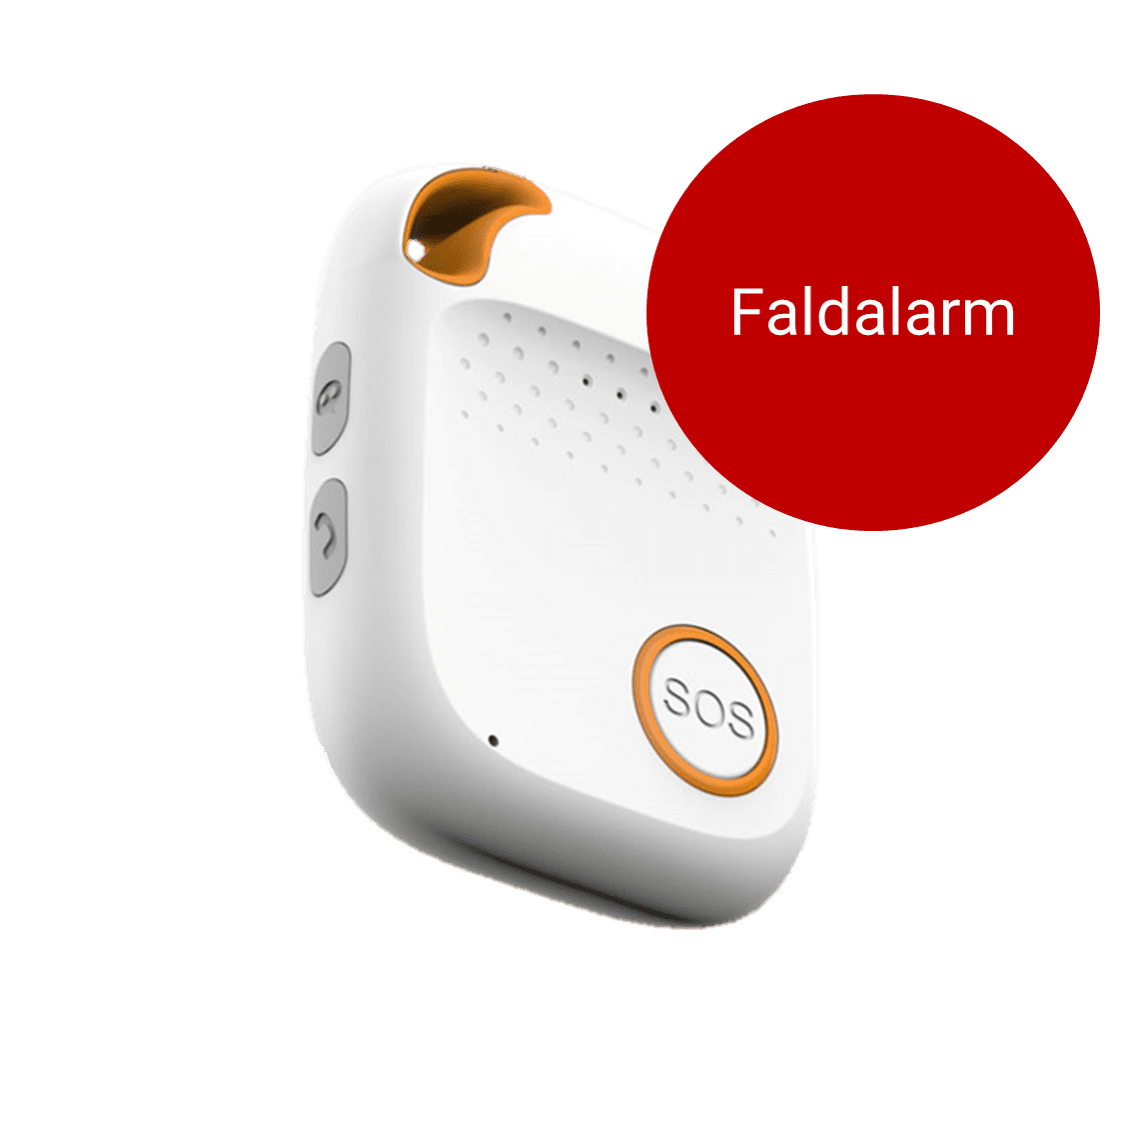
\includegraphics[width=0.5\linewidth]{report//images/faldalarm-cekura-go.png}
%     \caption{Cekura go 2.0}
%     \label{fig:cekura_go_20}
% \end{wrapfigure}



Cekura is a Danish company focused on products that connect to their emergency centre. Some of these products are their \textit{Cekura go 2.0}\cite{noauthor_ny_nodate} (as seen in \autoref{fig:cekura_go_20}) and \textit{emergency call jewel}\cite{noauthor_tryghedsalarm_nodate}. The \textit{emergency call jewel} is a necklace in which an emergency call button is positioned so that if there is an emergency, the wearer can quickly contact help, for example the Cekura emergency call centre. This product is made for elderly people who are in risk of falling, but also people who are impaired mobily, chronically sick or psychologically vulnerable. The\textit{ Cekura go 2.0} is similar and has an emergency button. However, it has a built-in function, in which it detects when a fall has occurred and automatically calls either the emergency call centre or a relative. The choice of who the emergency call button reaches out to is made when buying the product in the package chosen: either the relative, the call centre or the opportunity of choosing which one to call. 

\wrapimage{r}
    {report//images/faldalarm-cekura-go.png}
    {Cekura go 2.0}
    {cekura_go_20}

Besides previously mentioned features, the \textit{Cekura go 2.0 }has a built-in \gls{gps}, so that the wearer's exact location can be tracked. The \textit{emergency call jewel }does not have a \gls{gps}, but is sold alongside a \gls{gps}-tracker, so that the wearer’s location can be shared, if they bring the \gls{gps}-tracker with them. Both products have the possibility to speak through them, with the \textit{Cekura go 2.0} this feature is in the physical product, while this is only possible through the \gls{gps}-tracker with the \textit{emergency call jewel}. 

The \textit{emergency call jewel }is made with a design so that it looks like a normal piece of jewellery, this is meant for wearers' who feel stigmatised or who do not wish for acquintences to know that the wearer is wearing an emergency call. 
